\documentclass{article}
\usepackage{graphicx}
\usepackage{amsmath}

\setup{font=lm}
\title{Design Report: Design of Analog Integrated Circuits}
\date{2013-09-01}
\author{John Doe}

\begin{document}
  \maketitle
  \newpage
\section{Hand calculations}
\subsection{Settling error}
For the analysis of the settling error, the circuit digram as shown in the figure \ref{fig:amp_phase} has been used. 

\begin{figure}[h!]
  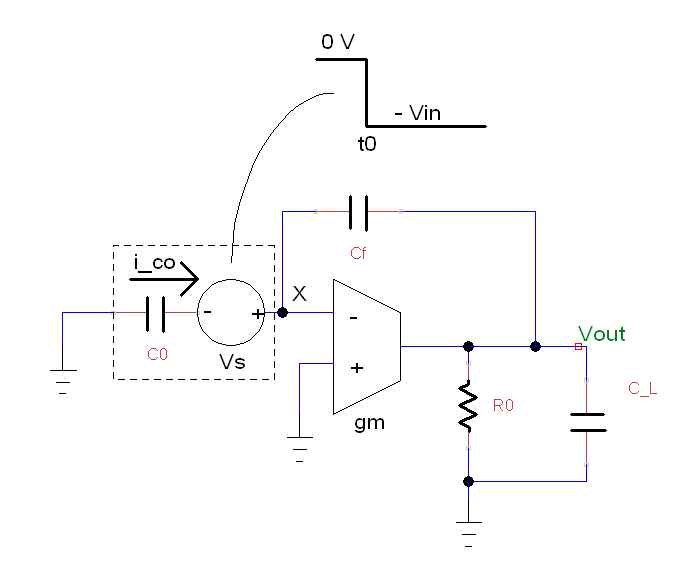
\includegraphics[width=\linewidth]{amplification_phase.png}
  \caption{During amplification phase}
  \label{fig:amp_phase}
\end{figure}

During the sampling phase, capacitor C0 is charged to $V_{in}$. At the beginning of the amplification phase, because he voltage across a capacitor cannot change simultaneously, there will be a negative step on node X. This can be represented as an ideal capacitor with a voltage source in series whose output in a negative going step as shown. The transfer fucntion $\frac{V_{out}}{V_s}(s)$ needs to be determined.
The current through the capacitor $C_o$ can be written as $i_{c0}=-\frac{V_x-V_s}{sC_0}$ \\
Also, 
	\begin{equation}
		(V_x-V_{out})sC_f = g_mV_x + V_{out}(\frac{1}{R_0} +sC_L) 
	\end{equation}
	\begin{equation*}
		V_{out}=V_x-\frac{i_{c0}}{sC_f}=V_x+\frac{(V_x-V_s)C_0}{C_f}
	\end{equation*}
The last equation can be re-written as
	\begin{equation}
		V_x=\frac{V_{out}+V_s\frac{C_0}{C_f}}{1+\frac{C_0}{C_f}}
	\end{equation}
Combining equations (1) and (2), the transfer function is derived as:
	\begin{equation}
		\frac{V_{out}}{V_s}(s) = \frac{\frac{-g_mC_0R_0}{g_mR_0C_f + C_0 +c_f}}{1+\frac{s(C_LC_0+C_LC_f+C_0C_f)R_0}{g_mR_0C_f + C_0 + C_f}}
	\end{equation}
The time constant of the settiling behavior, is thus given by
	\begin{equation}
		\tau=\frac{(C_LC_0+C_LC_f+C_0C_f)R_0}{g_mR_0C_f + C_0 + C_f}
	\end{equation}
Assuming that the duty cycle of the clock is 50\%, then there will be just half the period left for settling. Because it is a single pole system, the exprsssion for settling time can be derived simply as: 
Settling error =$ e^ {-\frac{1}{2f_{clk}\tau}}$
	\begin{equation}
	Error = e^ {-\frac{g_mR_0C_f + C_0 + C_f}{[(C_LC_0+C_LC_f+C_0C_f)R_0]2f_{clk}}}
	\end{equation}
An interesting observation ( not so if you think about it) is that the pole in the expression is approximated by: $ \frac{\beta gm}{C_L + C_0//C_f} $
The look in impedance (with the feedback network) is $\frac{1}{\beta g_m}$ and the total capacitance is indeed $C_L$ in parallel with the series combination of $C_0$ and $C_f$. 
However this expression is only valid for a single stage OTA. The settling of the internal node comes into picture. Because the pole at the output of the first stage is typically the lowest frequency, it may be a safe approximation to say that the internal node's GBW will limit the setling behavior. A detailed analysis of it can be found in \cite{4663680}. . \\ \\
However, for the simplicity of the design we approximated the settling time constant for settling as the inverse of GBW.
\section{Common Mode feedback}

In a fully differntial amplifer, where a current source is used as the load, there are two current sources in series. [encirled in figure \ref{fig:simple_ota1}].
\begin{figure}[h]
  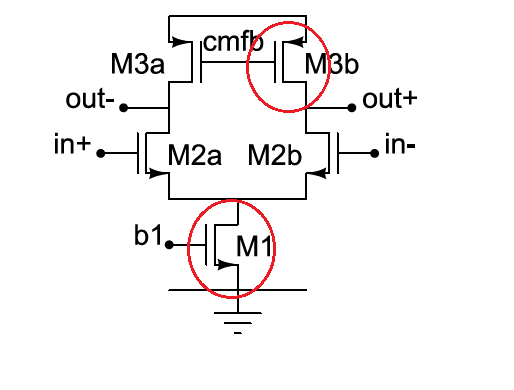
\includegraphics{simple_ota_cmfb.png}
  \caption{During amplification phase}
  \label{fig:simple_ota1}
\end{figure}
 Because of the high impedance of the current sources, the output common mode is not well defined. To define the output common mode, a CMFB circuit is used. A CMFB circuit senses the output common mode variation and changes the bias voltage of one of the current sources so that the output common mode is set to a fixed value. A CMFB circuit works in unity gain; \\
\begin{figure}[h!]
  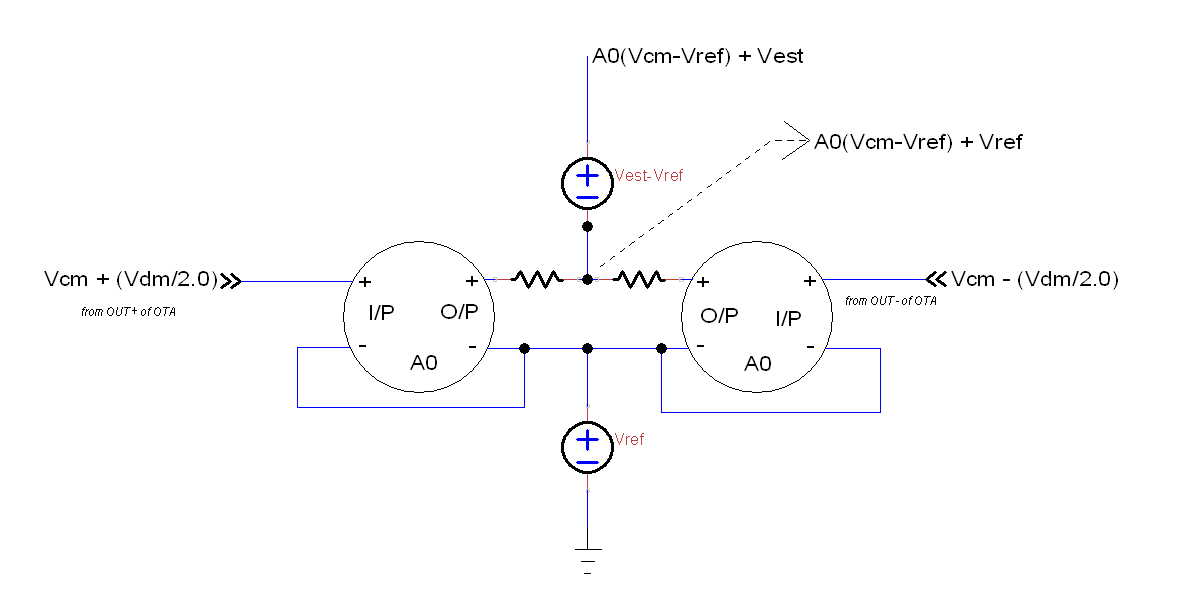
\includegraphics[width=\linewidth]{cmfb.png}
  \caption{During amplification phase}
  \label{fig:cmfb}
\end{figure}
An ideal CMFB circuit is shown in figure \ref{fig:cmfb}. The two resistors forms a voltage divider to cancel out the differential mode signals. The resistor along with the capacitance at the output of the CMFB circuit will define the GBW of the CMFB circuit. A CMFB circuit needs to be faster than the differential circuit. If it is slower, then it may be possible that the bias voltages are not stable. \\
The A0 in the circuit is (part) of open loop gain of the CMFB circuit. The other part of the gain comes from the transfer function from the output of the CMFB circuit to the node where the CMFB circuit is connected. In this case, larger the value of A0 is, smaller is the requirement on the accuracy of Vest. Vest is the estimated bias voltage of the current source that the CMFB will be driving. Vest does not need to be very accurate if A0 is large enough. \\
One of the problems seen during simulation if the simulator finds the solution as a large gate voltage which causes a large drain to gate current [basically a gate breakdown] but no drain to source current. In a real situation the voltage will be limited by the supply rails. The cmfb.cir netlist has been modified to reflect clamping of the output voltage to supply rails.
\bibliographystyle{unsrt}
\bibliography{reference}




\end{document}